%%%%%%%%%%%%%%%%%%%%%%%%%%%%%%%%%%%%%%%%%%%%%%%%%%%%%%%%%%%%%%%%%%%%%%%%%%%%%%%%%%%%%%%%%%%%%%%%%%%%%%%%%%%%%%%%%%%%%%
\chapter{Results}
%%%%%%%%%%%%%%%%%%%%%%%%%%%%%%%%%%%%%%%%%%%%%%%%%%%%%%%%%%%%%%%%%%%%%%%%%%%%%%%%%%%%%%%%%%%%%%%%%%%%%%%%%%%%%%%%%%%%%%
This chapter will contain a comparison between the different projection methods, and also with DM. Energy preservation with SLM is one of the primary concerns, but computation time, and difference between integration methods will also be mentioned.
\section{Convergence}%%%%%%%%%%%%%%%%%%%%%%%%%%%%%%%%%%%%%%%%%%%%%%%%%%%%%%%%%%%%%%%%%%%%%%%%%%%%%%%%%%%%%%%%%%%%%%%%%
This section will show convergence of all the methods, with both constant and varying energy. As a bonus, the energy will also be shown.

\subsection{Constant Energy}%%%%%%%%%%%%%%%%%%%%%%%%%%%%%%%%%%%%%%%%%%%%%%%%%%%%%%%%%%%%%%%%%%%%%%%%%%%%%%%%%%%%%%%
\begin{figure}[H]
        \centering
        \begin{subfigure}[b]{0.30\textwidth}
                \includegraphics[width=\textwidth]{../MATLAB/fig/intconv11.jpg}
                \caption{ Help line decreases with $k^2$. }
                \label{fig:intconv11}
        \end{subfigure}
        ~
        \begin{subfigure}[b]{0.30\textwidth}
                \includegraphics[width=\textwidth]{../MATLAB/fig/intconv12.jpg}
                \caption{ Help line decreases with $k$. }
                \label{fig:intconv12}
        \end{subfigure}
        \begin{subfigure}[b]{0.30\textwidth}
                \includegraphics[width=\textwidth]{../MATLAB/fig/intconv13.jpg}
                \caption{ Help line decreases with $k^2$. }
                \label{fig:intconv13}
        \end{subfigure}
        
        \begin{subfigure}[b]{0.30\textwidth}
                \includegraphics[width=\textwidth]{../MATLAB/fig/intener11.jpg}
                \caption{ Help line decreases with $k^2$. }
                \label{fig:intener11}
        \end{subfigure}
        ~
        \begin{subfigure}[b]{0.30\textwidth}
                \includegraphics[width=\textwidth]{../MATLAB/fig/intener12.jpg}
                \caption{ Help line decreases with $k$. }
                \label{fig:intener12}
        \end{subfigure}
        \begin{subfigure}[b]{0.30\textwidth}
                \includegraphics[width=\textwidth]{../MATLAB/fig/intener13.jpg}
                \caption{ Help line decreases with $k^2$. }
                \label{fig:intener13}
        \end{subfigure}        
        
\caption{Figure of the convergence for the different integration methods. Notice that forward Euler requires a much larger $k$ to obtain the same precision as the other methods. All methods converge with the expected rate. $n = 4$ and $\epsilon  = 1e-14$.}
\label{fig:intconv}
\end{figure}
It is clear from figure \ref{fig:intconv} and \ref{fig:intconv2} that all methods can be forced to have the same convergence if $\epsilon$ is chosen to be near machine accuracy.

Clearly forward Euler is not the iteration method you should use when you are concerned about the energy, but it does give the correct convergence rate, which is linear. \\

The other methods give a better approximation of the energy, and converges quadratically and near identically, as they should. The energy for all the methods is increasing, which is not desirable. This happens because more round off errors occur with larger $m$ and $k$, and when all these small numbers are added together to estimate the energy the become significant. \\

The reason for the small difference between midpoint and trapezoidal rule is that when the restart is performed midpoint rule is better at approximating the resulting error equation (the equation has non constant energy) than trapezoidal rule is. 

\subsection{Varying Energy}%%%%%%%%%%%%%%%%%%%%%%%%%%%%%%%%%%%%%%%%%%%%%%%%%%%%%%%%%%%%%%%%%%%%%%%%%%%%%%%%%%
\begin{figure}[H]
        \centering
        \begin{subfigure}[b]{0.30\textwidth}
                \includegraphics[width=\textwidth]{../MATLAB/fig/intconv21.jpg}
                %\includegraphics[width=\textwidth]{test}
                \caption{ Help line decreases with $k^2$. }
                \label{fig:intconv21}
        \end{subfigure}
        ~
        \begin{subfigure}[b]{0.30\textwidth}
                \includegraphics[width=\textwidth]{../MATLAB/fig/intconv22.jpg}
                %\includegraphics[width=\textwidth]{test}
                \caption{ Help line decreases with $k$. }
                \label{fig:intconv22}
        \end{subfigure}
        \begin{subfigure}[b]{0.30\textwidth}
                \includegraphics[width=\textwidth]{../MATLAB/fig/intconv23.jpg}
                %\includegraphics[width=\textwidth]{test}
                \caption{ Help line decreases with $k^2$. }
                \label{fig:intconv23}
        \end{subfigure}
        
                \begin{subfigure}[b]{0.30\textwidth}
                \includegraphics[width=\textwidth]{../MATLAB/fig/intener21.jpg}
                %\includegraphics[width=\textwidth]{test}
                \caption{ Help line decreases with $k^2$. }
                \label{fig:intener21}
        \end{subfigure}
        ~
        \begin{subfigure}[b]{0.30\textwidth}
                \includegraphics[width=\textwidth]{../MATLAB/fig/intener22.jpg}
                %\includegraphics[width=\textwidth]{test}
                \caption{ Help line decreases with $k$. }
                \label{fig:intener22}
        \end{subfigure}
        \begin{subfigure}[b]{0.30\textwidth}
                \includegraphics[width=\textwidth]{../MATLAB/fig/intener23.jpg}
                %\includegraphics[width=\textwidth]{test}
                \caption{ Help line decreases with $k^2$. }
                \label{fig:intener23}
        \end{subfigure}
\caption{Figure of the convergence for the different integration methods. Notice that forward Euler requires a much larger $k$ to obtain the same precision as the other methods. All methods converge with the expected rate. $n = 4$ and $\epsilon  = 1e-14$. All methods converge with the expected rate.}
\label{fig:intconv2}
\end{figure}

Forward Euler is running into some unexplainable problems with a sudden diverge at the last point. Though in this case it gives a nice convergence for both global energy and global error, except for the last point. \\

Trapezoidal rule and midpoint rule are again the better choices, with midpoint rule being slightly ahead. This is not a surprise since midpoint rule is a symplectic method while trapezoidal rule's good energy can be explained from is't quderatic convergence. \\

If you compare these figures to figure \ref{fig:intconv}, you will see that the energy is much higher in this case, but that they are decreasing, and not increasing. The reason for this is that the energy in figure \ref{fig:intconv2} is compared to the energy for the correct solution, while in figure \ref{fig:intconv} the energy is calculated, and not compared to anything. This gives a sort of bias and random answer, but is more useful than seeing how the energy changes for this case, or seeing how poorly the correct solution preserves energy.

!!!!!!!!!!!!!!!!!!!det må forklares et sted at trapezoidal ikke alltid er symplectisk men at midpouint alltid er det og at forward euler er ubrukelig (teoretisk altså)!!!!!!!!!!!!!!!!!!!!!!!!!!!!!\\

!!!!!!!!!!!!!!!!!!!!!!!!Skriv om noe om energiens konvergens når bildene er ferdige!!!!!!!!!!!!!!!!!\\

!!!!!!!!!!!!!!Kommentere litt at metodene fungerer i alle tilfeller!!!!!!!!!!!!!\\
\section{Integration method} %%%%%%%%%%%%%%%%%%%%%%%%%%%%%%%%%%%%%%%%%%%%%%%%%%%%%%%%%%%%%%%%%%%%%%%%%%%%%%%%%%%
%!!!!!!!!!!!!!!!!Burde det vært restart her også?!!!!!!!!!!!!!!!\\
This section will be concerned with comparing some different methods for integration in time. How well they estimate the error and energy will be the primary concern. \\
!!!!!!!!!!!!med eller uten restart?!!!!!!!!!!!!!!!!!!!!\\
\subsection{Constant energy with wave}%%%%%%%%%%%%%%%%%%%%%%%%%%%%%%%%%%%%%%%%%%%%%%%%%%%%%%%%%%%%%%%%%%%%%%%%%%%%%%%%%%%%%%%%%%

!!!!!!!!!!!!!!Skrive litt om hva denne konvergensen er!!!!!!!!!!!!!!!\\
\begin{figure}[H]
        \centering
        \begin{subfigure}[b]{0.30\textwidth}
                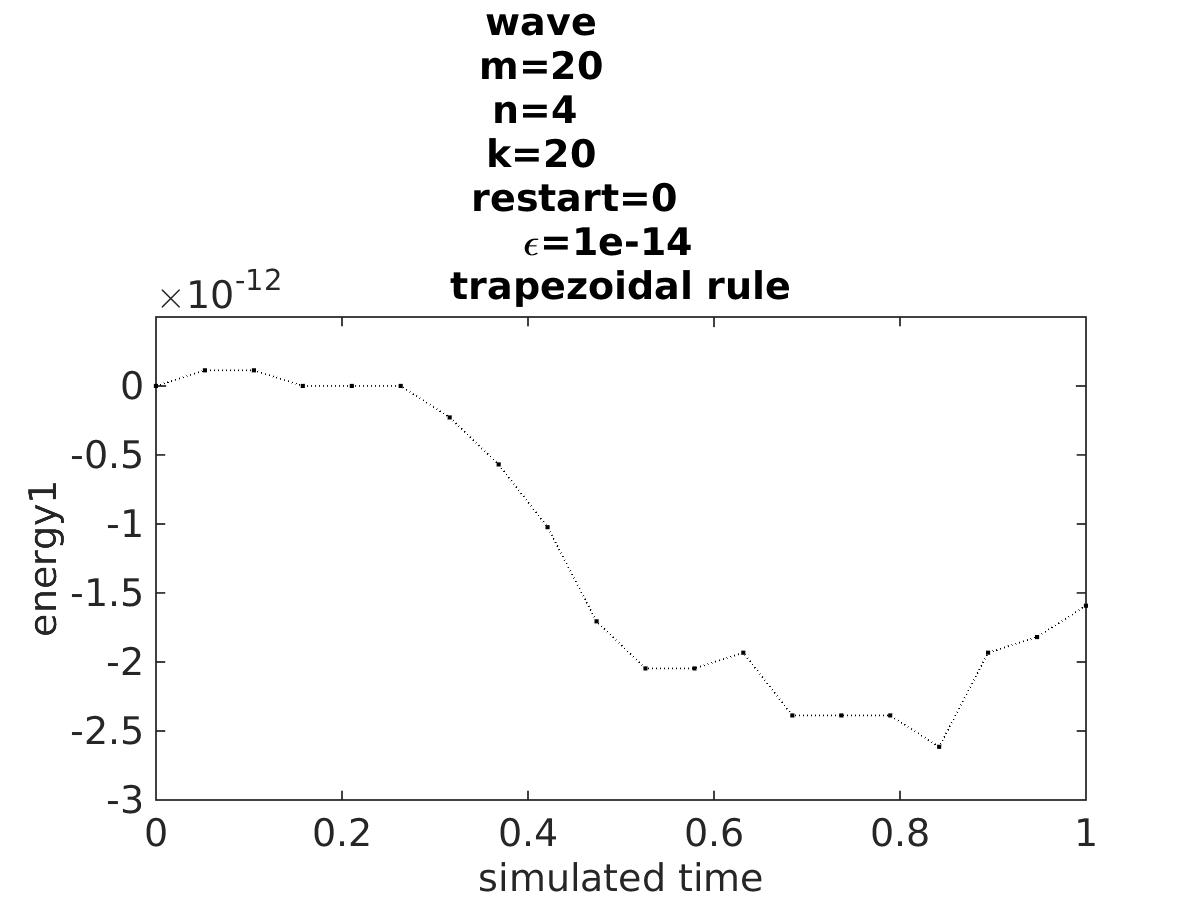
\includegraphics[width=\textwidth]{../MATLAB/fig/energyovertimetrapezoidal.jpg}
                \caption{ Energy with trapezoidal rule. }
                \label{fig:energyovertimetrapezoidal}
        \end{subfigure}%
        ~
        \begin{subfigure}[b]{0.30\textwidth}
                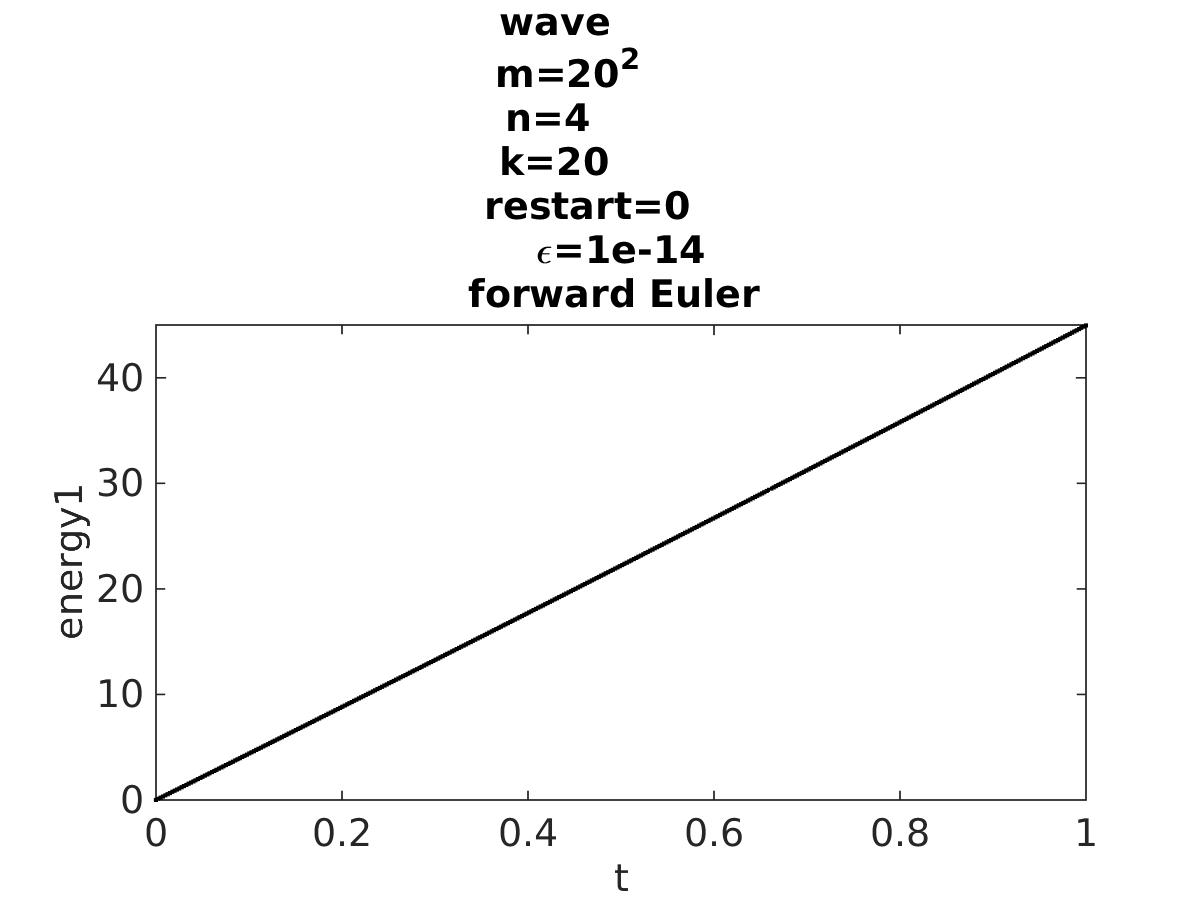
\includegraphics[width=\textwidth]{../MATLAB/fig/energyovertimeeuler.jpg}
                \caption{ Energy with forward Euler }
                \label{fig:energyovertimeeuler}
        \end{subfigure}
        \begin{subfigure}[b]{0.30\textwidth}
                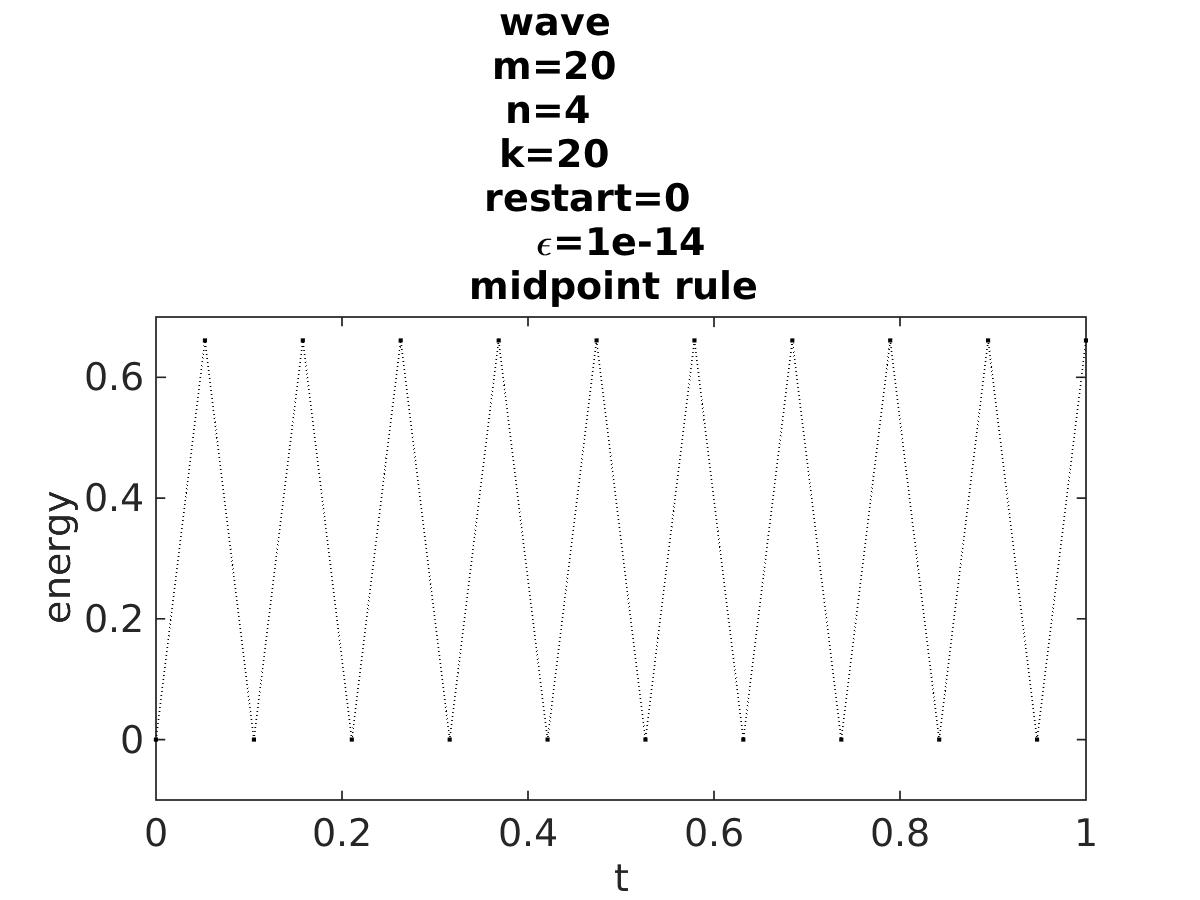
\includegraphics[width=\textwidth]{../MATLAB/fig/energyovertimemidpoint.jpg}
                \caption{ Energy with midpoint rule }
                \label{fig:energyovertimemidpoint}
        \end{subfigure}
        
        \begin{subfigure}[b]{0.30\textwidth}
                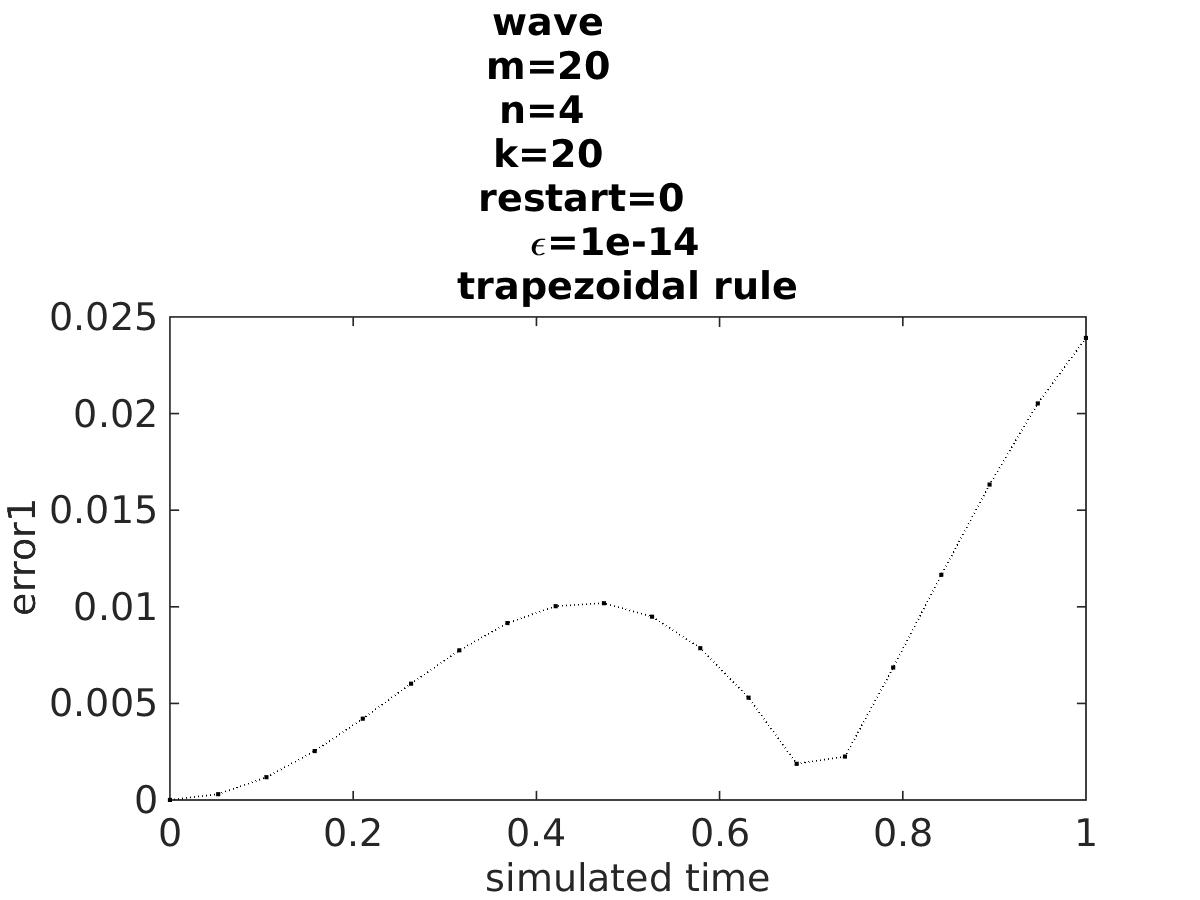
\includegraphics[width=\textwidth]{../MATLAB/fig/errorovertimetrapezoidal.jpg}
                \caption{ Error with trapezoidal rule }
                \label{fig:errorovertimetrapezoidal}
        \end{subfigure}%
        ~
        \begin{subfigure}[b]{0.30\textwidth}
                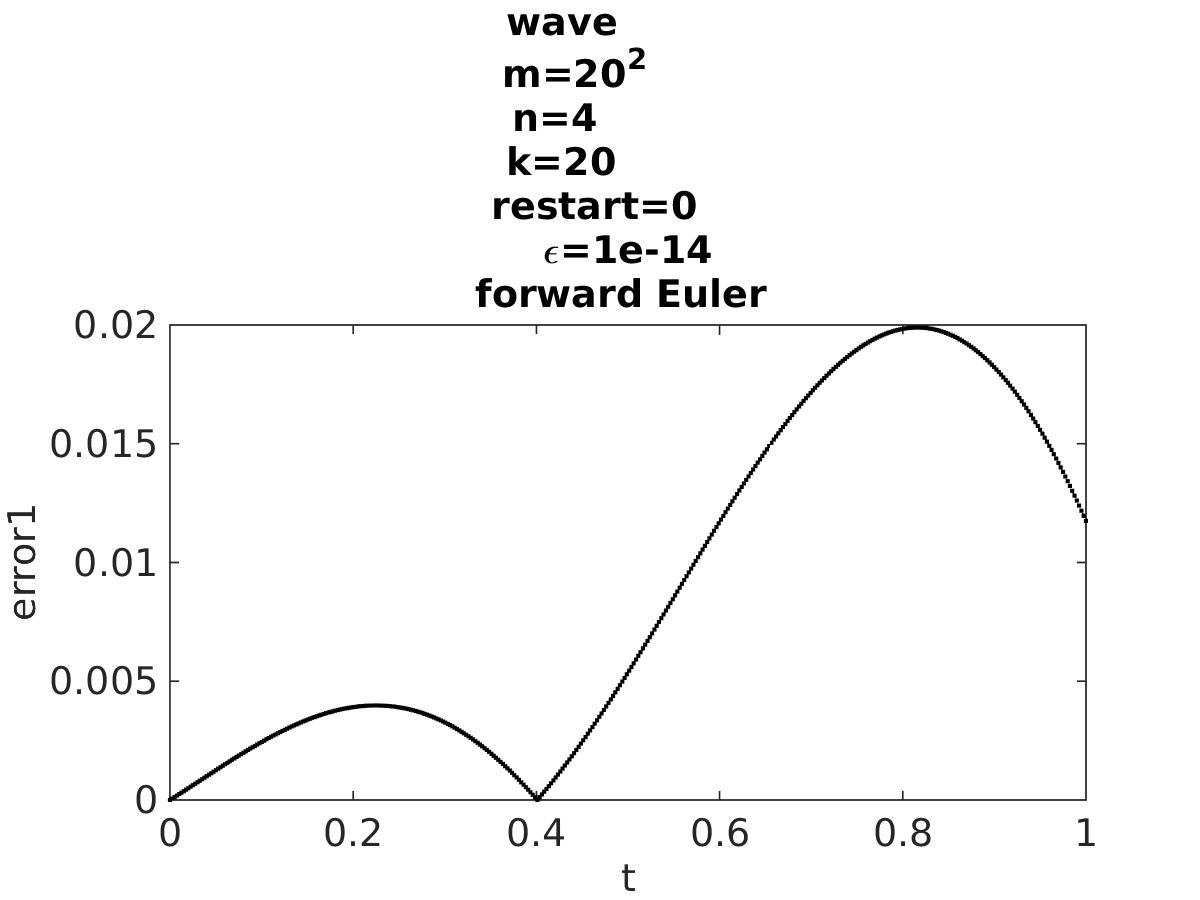
\includegraphics[width=\textwidth]{../MATLAB/fig/errorovertimeeuler.jpg}
                \caption{ Error with forward Euler }
                \label{fig:errorovertimeeuler}
        \end{subfigure}
        \begin{subfigure}[b]{0.30\textwidth}
                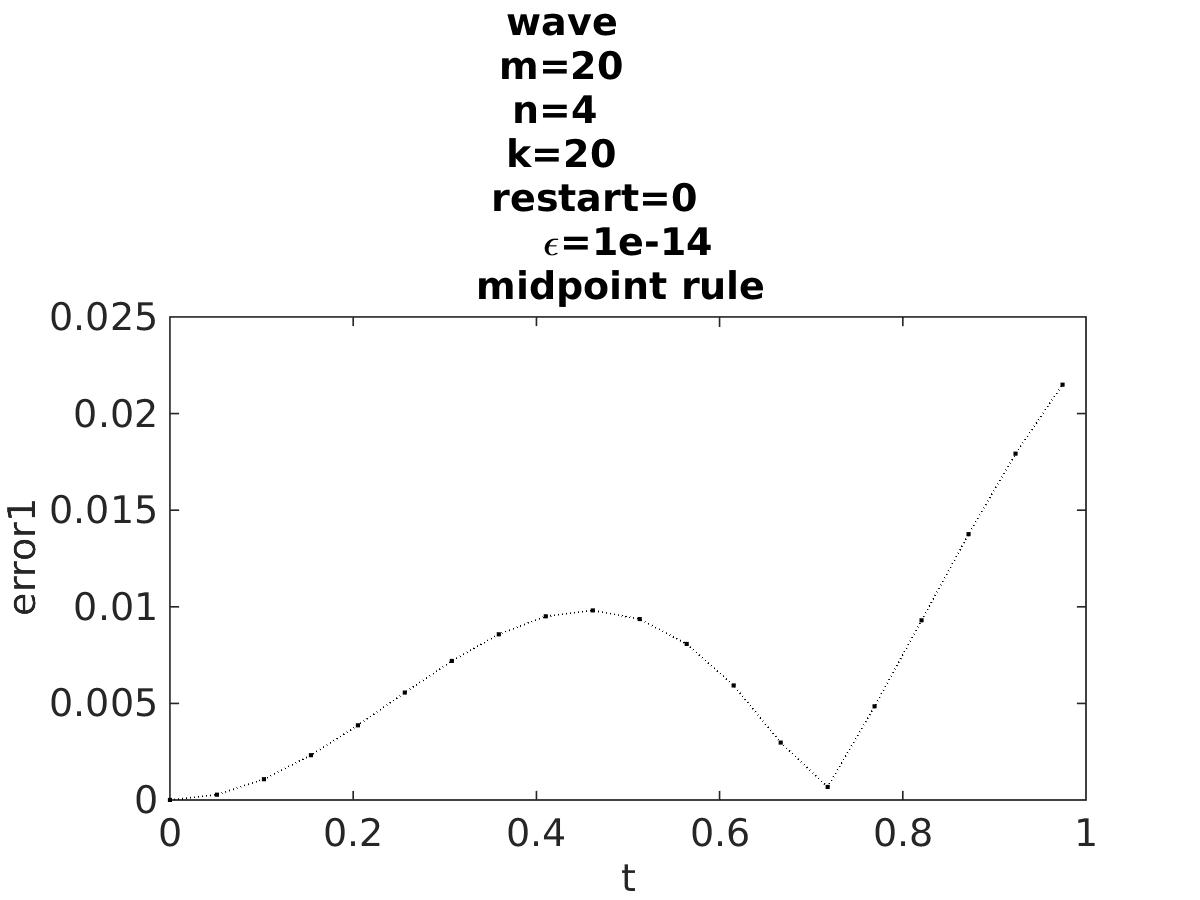
\includegraphics[width=\textwidth]{../MATLAB/fig/errorovertimemidpoint.jpg}
                \caption{ Error with midpoint rule }
                \label{fig:errorovertimemidpoint}
        \end{subfigure}
        \caption{A snapshot of how energy and error changes over the simulated time with the different integration method without restart. Notice that forward Euler requires a much larger $k$ to obtain the same precision as the other methods. $m = 20$, $n = 4$ $k=20$, restart is enabled with $\epsilon = 1e-14$.}
        \label{fig:error}
\end{figure}
Both trapezoidal rule and midpoint rule to gives a very precise estimation of energy and error. Forward Euler on the other hand gives a linearly increasing energy, and with that a larger error, making it useless as an integration method in this case. The reason for the wired shapes in figure \ref{fig:errorovertimetrapezoidal} and \ref{fig:errorovertimemidpoint} is the periodicity of the test problem. 

Forward Euler gives a good approximation of the error, but since the energy is linearly increasing it should not be used together with SLPM. \\

Trapezoidal rule and midpoint rule behaves very similar, with midpoint rule having a small advantage again because of the restart.

!!!!!!!!!!!!!!!Skrive at disse bildene er laget på en annen måte enn de andre!!!!!!!!!!!!\\
\subsection{Varying energy with waves}%%%%%%%%%%%%%%%%%%%%%%%%%%%%%%%%%%%%%%%%%%%%%%%%%%%%%%%%%%%%%%%%%%%%%%%%%%%%%%%%%%%%%%%%%%%

\begin{figure}[H]
        \centering
        \begin{subfigure}[b]{0.30\textwidth}
                \includegraphics[width=\textwidth]{../MATLAB/fig/energychangtimetrapezoidal.jpg}
                \caption{ Energy with trapezoidal rule. }
                \label{fig:energychangtimetrapezoidal}
        \end{subfigure}%
        ~
        \begin{subfigure}[b]{0.30\textwidth}
                \includegraphics[width=\textwidth]{../MATLAB/fig/energychangtimeeuler.jpg}
                \caption{ Energy with forward Euler. }
                \label{fig:energychangtimeeuler}
        \end{subfigure}
        \begin{subfigure}[b]{0.30\textwidth}
                \includegraphics[width=\textwidth]{../MATLAB/fig/energychangtimemidpoint.jpg}
                \caption{ Energy with midpoint rule. }
                \label{fig:energychangtimemidpoint}
        \end{subfigure}
        
        \begin{subfigure}[b]{0.30\textwidth}
                \includegraphics[width=\textwidth]{../MATLAB/fig/errorchangtimetrapezoidal.jpg}
                \caption{ Error with trapezoidal rule. }
                \label{fig:errorchangtimetrapezoidal}
        \end{subfigure}%
        ~
        \begin{subfigure}[b]{0.30\textwidth}
                \includegraphics[width=\textwidth]{../MATLAB/fig/errorchangtimeeuler.jpg}
                \caption{ Error with forward Euler. }
                \label{fig:errorchangtimeeuler}
        \end{subfigure}
        \begin{subfigure}[b]{0.30\textwidth}
                \includegraphics[width=\textwidth]{../MATLAB/fig/errorchangtimemidpoint.jpg}
                \caption{ Error with midpoint rule rule. }
                \label{fig:errorchangtimemidpoint}
        \end{subfigure}
        \caption{A snapshot of how energy and error changes over the simulated time with the different integration method without restart.\\$\neptune$}
        \label{fig:errorchang}
\end{figure}
In this case all methods gives a suitable convergence for the error and the energy. There is no longer any problems with forward Euler's increasing energy. Again the shapes on the figures is a property of the test problems, and not a flaw in the method.

Again midpoint rule performs better. From here on, forward Euler will no longer be used due to its poor energy preserving properties. Trapezoidal rule will be used when the energy is constant, though midpoint gives a better approximation. The reason for this is that there is no huge difference between trapezoidal rule and midpoint rule when the energy is constant, trapezoidal rule is also a bit faster. When the energy is not constant midpoint rule will be used. 

\section{How to choose $\epsilon$} %%%%%%%%%%%%%%%%%%%%%%%%%%%%%%%%%%%%%%%%%%%%%%%%%%%%%%%%%%%%%%%%%%%%%%%%%%%%%%%%%%%%%
This section will look at how the different projection methods compare to each other in relation to error, energy and time consumption. There will also be a comparison between restart variable and computation time. 

%\subsection{}


\subsection{Constant energy} \label{sec:SLMconstant}%%%%%%%%%%%%%%%%%%%%%%%%%%%%%%%%%%%%%%%%%%%%%%%%%%%%%%%%%%%%%%%%%%
!!!!!!!!!!!!!!!!!!!!!Det må skrives en del mer i dette kapitelet!!!!!!!!!!!!!!!!!!!!!!\\

\begin{figure}[H]
        \centering
        
		\begin{subfigure}[b]{0.3\textwidth}
                \includegraphics[width=\textwidth]{../MATLAB/fig/compareEnergyw.jpg}
                \caption{ Energy. }
                \label{fig:compareEnergyw}
        \end{subfigure}
        ~
        \begin{subfigure}[b]{0.3\textwidth}
                \includegraphics[width=\textwidth]{../MATLAB/fig/compareErrorw.jpg}
                \caption{ Error. }
                \label{fig:compareErrorw}
        \end{subfigure}
        ~
        \begin{subfigure}[b]{0.3\textwidth}
                \includegraphics[width=\textwidth]{../MATLAB/fig/compareIterw.jpg}
                \caption{ Number of restarts.  }
                \label{fig:compareIterw}
        \end{subfigure}
        
        \begin{subfigure}[b]{0.3\textwidth}
                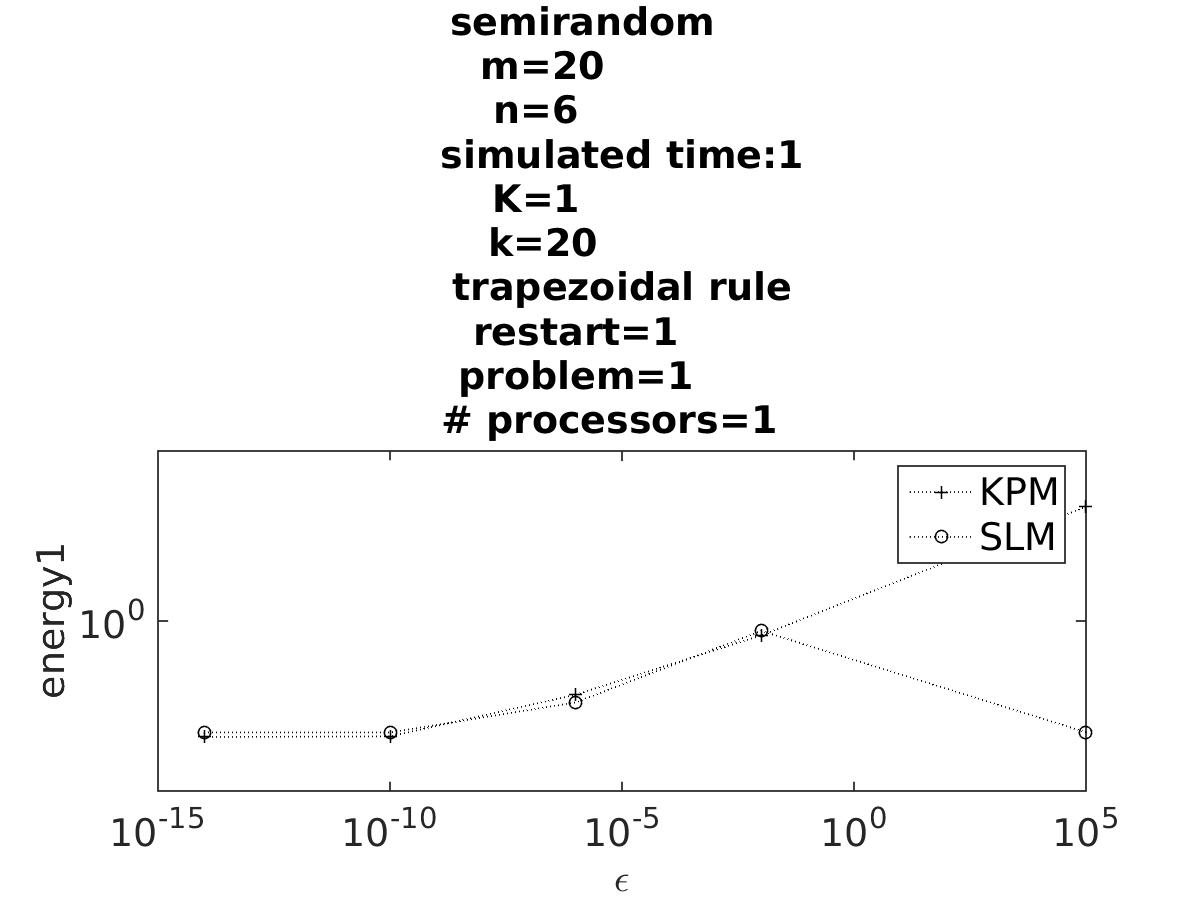
\includegraphics[width=\textwidth]{../MATLAB/fig/compareEnergy.jpg}
                \caption{Energy.}
                \label{fig:compareEnergy}
        \end{subfigure}
        ~
        \begin{subfigure}[b]{0.3\textwidth}
                \includegraphics[width=\textwidth]{../MATLAB/fig/compareError.jpg}
                \caption{ Error. }
                \label{fig:compareError}
        \end{subfigure}
        ~
        \begin{subfigure}[b]{0.3\textwidth}
                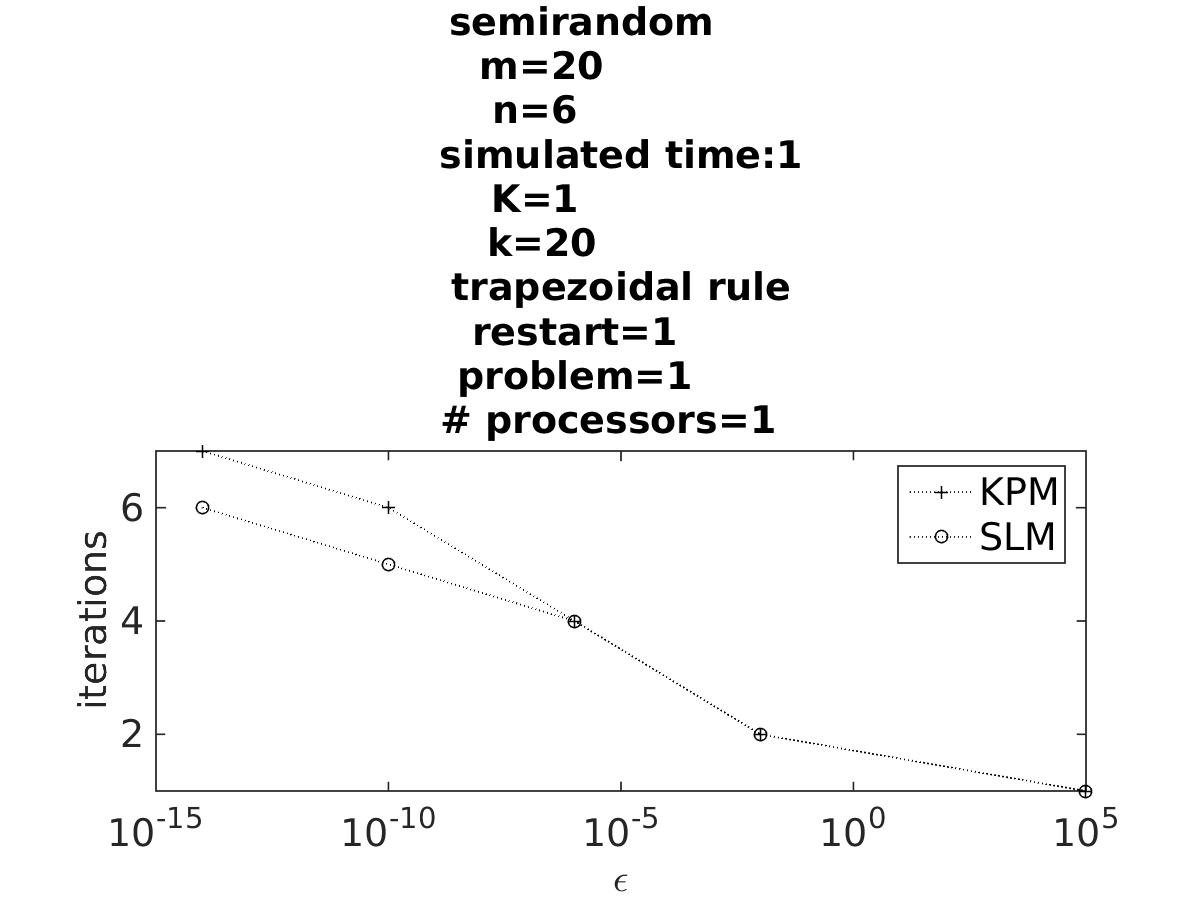
\includegraphics[width=\textwidth]{../MATLAB/fig/compareIter.jpg}
                \caption{ Number of restarts.  }
                \label{fig:compareIter}
        \end{subfigure}
        \caption{ The figure shows how the different methods change the energy and error with different number of restart for \texttt{semirandom}.  }
        \label{fig:compare}
\end{figure}



There is a clear difference between how well the energy is estimated for \texttt{wave} and \texttt{semirandom}. For \texttt{semirandom} there is not much difference between SLM and Arnoldi, although SLM seams to give a slight better approximation than Arnoldi. With \texttt{semirandom} at $\epsilon = 10^{-10}$ Arnoldi preforms one more iteration than SLM, which makes it give a better approximation, aside from that SLM consistently preform better than Arnoldi.\\
When comparing figure \ref{fig:compare} and figure \ref{fig:comparew} it is important to remember that the way the $er_1$ and $er_2$ is found is very differently, and that might explain the why the cases differs so much. But the difference might also be explained with \texttt{semiradom} being a much harder equation to solve.\\
!!!!!!!!!!!!!Skriv litt mer om hvorfor bildene for semirandom og wave er så forksjelkige!!!!!!!!!!!!!!!!!!!!!\\

\subsection{Varying energy}%%%%%%%%%%%%%%%%%%%%%%%%%%%%%%%%%%%%%%%%%%%%%%%%%%%%%%%%%%%%%%%%%%%%%%%%%%%%%%%%%%%%%%%%%%%


\begin{figure}[H]
        \centering
        
        \begin{subfigure}[b]{0.3\textwidth}
                \includegraphics[width=\textwidth]{../MATLAB/fig/compareEnergy2w.jpg}
                \caption{ The difference in energy with and without restart. }
                \label{fig:compareEnergy2w}
        \end{subfigure}
        ~
        \begin{subfigure}[b]{0.3\textwidth}
                \includegraphics[width=\textwidth]{../MATLAB/fig/compareError2w.jpg}
                \caption{ The difference in energy with and without restart. }
                \label{fig:compareError2w}
        \end{subfigure}
        ~
        \begin{subfigure}[b]{0.3\textwidth}
                \includegraphics[width=\textwidth]{../MATLAB/fig/compareIter2w.jpg}
                \caption{ The number of iterations performed with and without restarting.  }
                \label{fig:compareIter2w}
        \end{subfigure}
        
        \begin{subfigure}[b]{0.3\textwidth}
                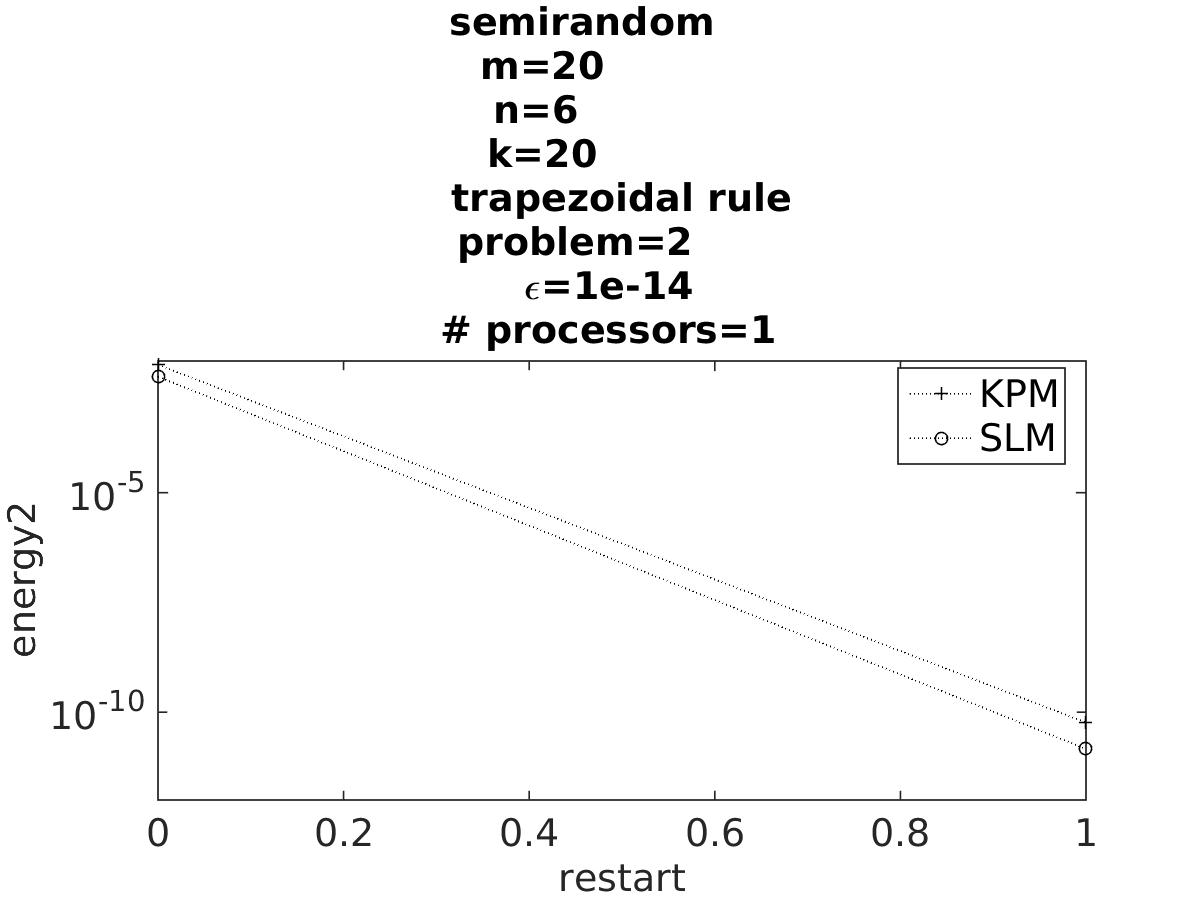
\includegraphics[width=\textwidth]{../MATLAB/fig/compareEnergy2.jpg}
                \caption{ The difference in energy with and without restart. }
                \label{fig:compareEnergy2}
        \end{subfigure}
        ~
        \begin{subfigure}[b]{0.3\textwidth}
                \includegraphics[width=\textwidth]{../MATLAB/fig/compareError2.jpg}
                \caption{ The difference in energy with and without restart. }
                \label{fig:compareError2}
        \end{subfigure}
        ~
        \begin{subfigure}[b]{0.3\textwidth}
                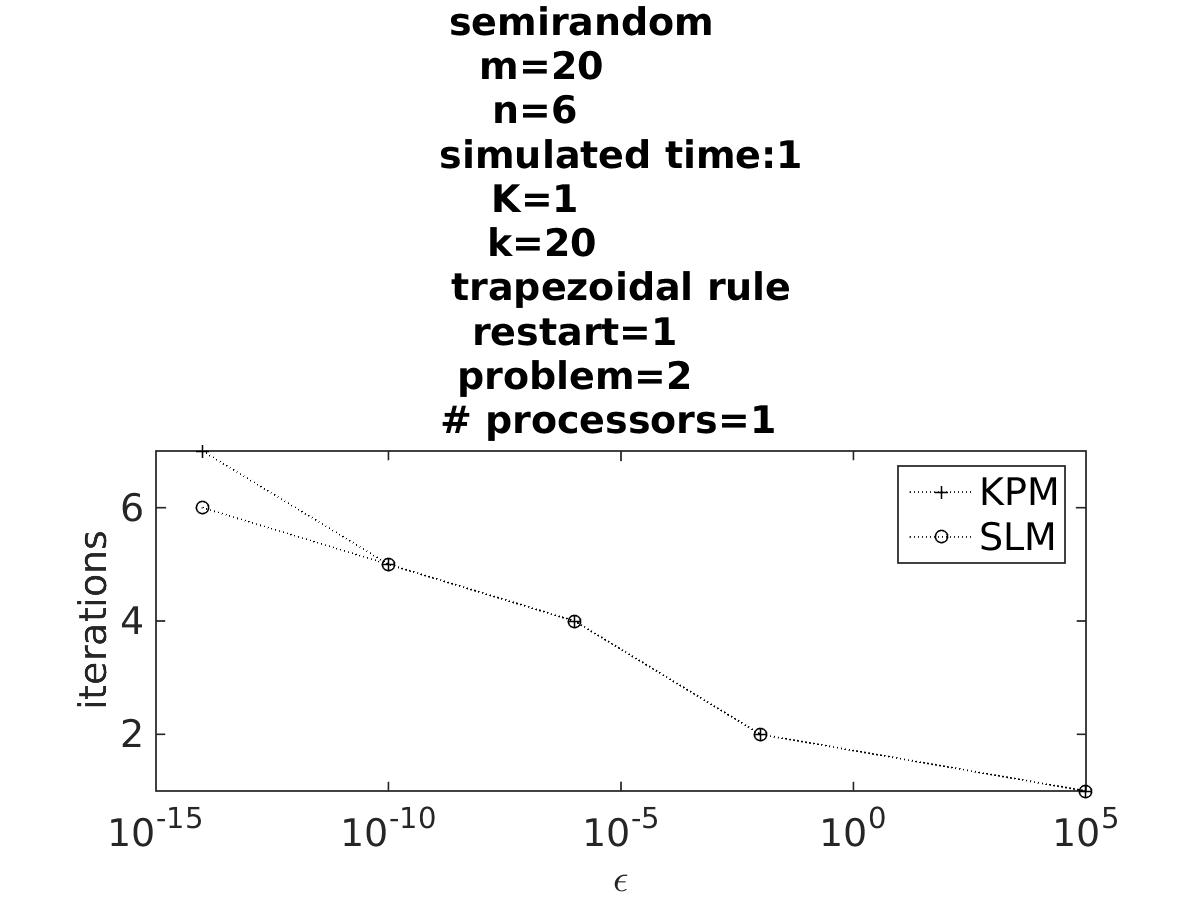
\includegraphics[width=\textwidth]{../MATLAB/fig/compareIter2.jpg}
                \caption{ The number of iterations performed with and without restarting.  }
                \label{fig:compareIter2}
        \end{subfigure}
        \caption{ The figure shows how the different methods change the energy and error with different number of restart for \texttt{wave}.  }
        \label{fig:compare2}
\end{figure}


The results here are very similar to the results found in section \ref{sec:SLMconstant}, except that the energy and error changes for the first points for both SLM and Arnoldi. SLM still gives the better approximation.

\subsection{A rule based for $\epsilon$}

\begin{figure}[H]
        \centering
        
        \begin{subfigure}[b]{0.3\textwidth}
                \includegraphics[width=\textwidth]{../MATLAB/fig/ruleerr.jpg}
                \caption{ !!!!!!!!!!!!!!!!!!!!!!!!! }
                \label{fig:ruleerr}
        \end{subfigure}
        ~
        \begin{subfigure}[b]{0.3\textwidth}
                \includegraphics[width=\textwidth]{../MATLAB/fig/ruleener.jpg}
                \caption{ !!!!!!!!!!!!!!!!!!!!!!! }
                \label{fig:ruleener}
        \end{subfigure}
        ~
        \begin{subfigure}[b]{0.3\textwidth}
                \includegraphics[width=\textwidth]{../MATLAB/fig/ruleiter.jpg}
                \caption{ !!!!!!!!!!!!!!!!!!!!  }
                \label{fig:ruleiter}
        \end{subfigure}
        
		\begin{subfigure}[b]{0.3\textwidth}
                \includegraphics[width=\textwidth]{../MATLAB/fig/ruleerr1.jpg}
                \caption{ !!!!!!!!!!!!!!!!!!!!!!!!! }
                \label{fig:ruleerr1}
        \end{subfigure}
        ~
        \begin{subfigure}[b]{0.3\textwidth}
                \includegraphics[width=\textwidth]{../MATLAB/fig/ruleener1.jpg}
                \caption{ !!!!!!!!!!!!!!!!!!!!!!! }
                \label{fig:ruleener1}
        \end{subfigure}
        ~
        \begin{subfigure}[b]{0.3\textwidth}
                \includegraphics[width=\textwidth]{../MATLAB/fig/ruleiter1.jpg}
                \caption{ !!!!!!!!!!!!!!!!!!!!  }
                \label{fig:ruleiter1}
        \end{subfigure}
        \caption{ The figure shows how the different methods change the energy and error with different number of restart for \texttt{wave}.  }
        \label{fig:rule}
\end{figure}

\section{Energy and error }%%%%%%%%%%%%%%%%%%%%%%%%%%%%%%%%%%%%%%%%%%%%%%%%%%%%%%%%%%%%%%%%%%%%%%%%%%%%%%%%%%%%%
%It can be proved that a restart of SLM does not alter the energy \cite{luli}. This section is devoted to seeing holds with numerical approximations. \\

Since SLM gives a symplectic matrix, the energy should not change with time, and the error should increase linearly with time. This section will be devoted to seeing how well this works in practice. There will also be a comparison about how the restart changes the energy preservation. In addition we will see if there is much difference if the energy is constant or varying.

\subsection{Constant energy} %%%%%%%%%%%%%%%%%%%%%%%%%%%%%%%%%%%%%%%%%%%%%%%%%%%%%%%%%%%%%%%%%%%%%%%%%%%%%%%%%%%%%%%%%%%%

\subsubsection{Energy and error without restart} %%%%%%%%%%%%%%%%%%%%%%%%%%%%%%%%%%%%%%%%%%%%%%%%%%%%%%%%%%%%%%%%%%%%%%%%%%%%%%%

\begin{figure}[H]
        \centering
        \begin{subfigure}[b]{0.45\textwidth}
                \includegraphics[width=\textwidth]{../MATLAB/fig/SLMenergyw.jpg}
                \caption{Global error for \texttt{wave}.}
                \label{fig:SLMenergyw}
        \end{subfigure}
        ~
        \begin{subfigure}[b]{0.45\textwidth}
                \includegraphics[width=\textwidth]{../MATLAB/fig/SLMerrorw.jpg}
                \caption{Global energy for \texttt{wave}. }
                \label{fig:SLMerrorw}
        \end{subfigure}
        
        \begin{subfigure}[b]{0.45\textwidth}
                \includegraphics[width=\textwidth]{../MATLAB/fig/SLMenergys.jpg}
                \caption{Global error for \texttt{semirandom}.}
                \label{fig:SLMenergys}
        \end{subfigure}
		~
        \begin{subfigure}[b]{0.45\textwidth}
                \includegraphics[width=\textwidth]{../MATLAB/fig/SLMerrors.jpg}
                \caption{Global energy for \texttt{semirandom}.}
                \label{fig:SLMerrors}
        \end{subfigure}
        \caption{ The figure shows how the global energy and global error changes as a function of simulated time, without restart. $m = 20$, $n = 8$ and trapezoidal rule is used to integrate.}
        \label{fig:SLMenergyerror}
\end{figure}
The figures shows no or small differences between the global error for KPM and SLPM. It is clear that DM gives a better approximation than the other two methods, but not by far, and this is without restart. Regarding energy I think figure \ref{fig:SLMenergys} shows it best. KPM is clearly not the best orthogonalisation method when it comes to estimating energy. 

\subsubsection{Energy and error with restart} %%%%%%%%%%%%%%%%%%%%%%%%%%%%%%%%%%%%%%%%%%%%%%%%%%%%%%%%%%%%%%%%%%%%%%%%%%%
\begin{figure}[H]
        \centering
        \begin{subfigure}[b]{0.45\textwidth}
                \includegraphics[width=\textwidth]{../MATLAB/fig/SLMenergyw1.jpg}
                \caption{Global error for \texttt{wave}.}
                \label{fig:SLMenergyw1}
        \end{subfigure}
        ~
        \begin{subfigure}[b]{0.45\textwidth}
                \includegraphics[width=\textwidth]{../MATLAB/fig/SLMerrorw1.jpg}
                \caption{Global energy for \texttt{wave}.}
                \label{fig:SLMerrorw1}
        \end{subfigure}
        
        \begin{subfigure}[b]{0.45\textwidth}
                \includegraphics[width=\textwidth]{../MATLAB/fig/SLMenergys1.jpg}
                \caption{Global error for \texttt{semirandom}.}
                \label{fig:SLMenergys1}
        \end{subfigure}
		~
        \begin{subfigure}[b]{0.45\textwidth}
                \includegraphics[width=\textwidth]{../MATLAB/fig/SLMerrors1.jpg}
                \caption{Global energy for \texttt{semirandom}.}
                \label{fig:SLMerrors1}
        \end{subfigure}
        \caption{ The figure shows how the global energy and global error changes as a function of simulated time with restart. $m = 20$, $n = 8$ and trapezoidal rule is used to integrate.}
        \label{fig:SLMenergyerror1}
\end{figure}
This picture shows some of the biggest weakness of the orthogonalisation methods I have  uncovered. The restart! The reason for the incredible increase on the energy is due to the fact that when restart is enabled the system is no longer symplctic, and thus the energy is no longer constant, and every restart changes the energy creating a feedback loop. \\ 

The good news on the other hand is that if $\epsilon$ is kept small enough the error will not diverge. SLPM also seams to be better at maintaining a small error, probably because of a smaller increase in energy. 

\subsection{Varying energy}
The focus has till now been to look at how the methods work when the energy is constant. This section will show how the methods work when the energy is varying. 

\subsubsection{Energy and error without restart}%%%%%%%%%%%%%%%%%%%%%%%%%%%%%%%%%%%%%%%%%%%%%%%%%%%%%%%%%%%%%%%%%%%%%%

\begin{figure}[H]
        \centering
        \begin{subfigure}[b]{0.45\textwidth}
                \includegraphics[width=\textwidth]{../MATLAB/fig/SLMenergyw3.jpg}
                \caption{Global error for \texttt{wave} without restart.}
                \label{fig:SLMenergyw1}
        \end{subfigure}
        ~
        \begin{subfigure}[b]{0.45\textwidth}
                \includegraphics[width=\textwidth]{../MATLAB/fig/SLMerrorw3.jpg}
                \caption{Global energy for \texttt{wave} without restart.}
                \label{fig:SLMerrorw1}
        \end{subfigure}
        
        \begin{subfigure}[b]{0.45\textwidth}
                \includegraphics[width=\textwidth]{../MATLAB/fig/SLMenergys3.jpg}
                \caption{Global error for \texttt{wave} with restart.}
                \label{fig:SLMenergys1}
        \end{subfigure}
		~
        \begin{subfigure}[b]{0.45\textwidth}
                \includegraphics[width=\textwidth]{../MATLAB/fig/SLMerrors3.jpg}
                \caption{Global energy for \texttt{wave} with restart.}
                \label{fig:SLMerrors1}
        \end{subfigure}
        \caption{!!!!!!!!!!!!!!!!Skriv noe her!!!!!!!!!!!!!!! og på alle subcaptioner!!!!!!!!}
        \label{fig:SLMenergyerror1}
\end{figure}
In this case there is no difference between the projection methods. DM performs marginally better than the other methods, but not asymptotically better, there seams to be a constant difference between the two methods, probably depending on $n$, where a larger $n$ would give a smaller difference.
!!!!!!!!!!!!!!!!!!!!Skriv noe!!!!!!!!!!!!!!!!!!!!!!!!!!!!!!\\
\subsubsection{Energy and error with restart}%%%%%%%%%%%%%%%%%%%%%%%%%%%%%%%%%%%%%%%%%%%%%%%%%%%%%%%%%%%%%%%%%%%%%%%%%

\begin{figure}[H]
        \centering
        \begin{subfigure}[b]{0.45\textwidth}
                \includegraphics[width=\textwidth]{../MATLAB/fig/SLMenergyw13.jpg}
                \caption{Global error for \texttt{wave} without restart.}
                \label{fig:SLMenergyw13}
        \end{subfigure}
        ~
        \begin{subfigure}[b]{0.45\textwidth}
                \includegraphics[width=\textwidth]{../MATLAB/fig/SLMerrorw13.jpg}
                \caption{Global energy for \texttt{wave} without restart.}
                \label{fig:SLMerrorw13}
        \end{subfigure}
        
        \begin{subfigure}[b]{0.45\textwidth}
                \includegraphics[width=\textwidth]{../MATLAB/fig/SLMenergys13.jpg}
                \caption{Global error for \texttt{wave} with restart.}
                \label{fig:SLMenergys13}
        \end{subfigure}
		~
        \begin{subfigure}[b]{0.45\textwidth}
                \includegraphics[width=\textwidth]{../MATLAB/fig/SLMerrors13.jpg}
                \caption{Global energy for \texttt{wave} with restart.}
                \label{fig:SLMerrors13}
        \end{subfigure}
        \caption{!!!!!!!!!!!!!!!!Skriv noe her!!!!!!!!!!!!!!! og på alle subcaptioner!!!!!!!!}
        \label{fig:SLMenergyerror13}
\end{figure}

Both SLPM and KPM does an equally poor job at approximating the solution when restart is enabled. An interesting event is the step happening in figure \ref{fig:SLMerrorw13}, this is the point where the energy starts to diverge. Another interesting thing about that is that KPM never seams to increase with the same rate as SLPM. So for longer times it seams that SLPM does not always have an advantage over KPM. But if you look closely you will see that the energy for SLPM is initially much smaller for KPM.

\subsection{Constant energies with SLM} %%%%%%%%%%%%%%%%%%%%%%%%%%%%%%%%%%%%%%%%%%%%%%%%%%%%%%%%%%%%%%%%%%%%%%%%%%%%%%%%%
Some theoretical results was presented for me by Lu Li. The theory can be found in \cite{!!!!!!!!!!!!}. In short she predicted that the global energy of SLPM should be constant when restart is not enabled, in addition to energy $\mathcal{H}_3 $ and $\mathcal{H}_4$ being constant. An other important result would be to see if the global energy is constant when restart is enabled. These question will be answered in this section. 

\subsubsection{Energy of SLM without restart}%%%%%%%%%%%%%%%%%%%%%%%%%%%%%%%%%%%%%%%%%%%%%%%%%%%%%%%%%%%%%%%%%%%%%%%%%

\begin{figure}[H]
        \centering
        \begin{subfigure}[b]{0.45\textwidth}
                \includegraphics[width=\textwidth]{../MATLAB/fig/SLMconstew.jpg}
                \caption{Global energy for \texttt{wave} without restart.}
                \label{fig:SLMconstew}
        \end{subfigure}
        ~
        \begin{subfigure}[b]{0.45\textwidth}
                \includegraphics[width=\textwidth]{../MATLAB/fig/SLMconstewtrap.jpg}
                \caption{Global energy for \texttt{semirandom} without restart.}
                \label{fig:SLMconstes}
        \end{subfigure}

        \caption{The change in energy for functions that should have constant energy. $m = 20$, $n = 4$, trapezoidal rule}
        \label{fig:SLMconste}
\end{figure}
When I look at the figure I would say that it is clear that the energy is not constant for either SLPM or DM. But DM is a symplectic method! It uses a Hamiltonian matrix, and a symplectic integrator, So why does it increase? My guess would be small round off errors that when summed up enough becomes considerable large. So this explains why DM has a small increase. But what about SLPM, my guess is that the increase in energy not is actually that much bigger, it changes more, both up and down, but if you look at the first and last point it is actually about the same increase as DM has. The increase in energy is in any case much smaller than the linear increase a non-symplecitc method would have. It seams close enough for me, and I conclude that SLPM is energy preserving, with a symplectic integrator.

%!!!!!!!!!!!!!!!!!!!!!!!!Bilde til høyre er ubrukelig!!!!!!!!!!!!!!!!\\
\subsubsection{Energy og SLM with restart} %%%%%%%%%%%%%%%%%%%%%%%%%%%%%%%%%%%%%%%%%%%%%%%%%%%%%%%%%%%%%%%%%%%%%%%%%%%
\begin{figure}[H]
        \centering
        \begin{subfigure}[b]{0.45\textwidth}
                \includegraphics[width=\textwidth]{../MATLAB/fig/SLMconstewr.jpg}
                \caption{Global error for \texttt{wave} without restart.}
                \label{fig:SLMconstewr}
        \end{subfigure}
        ~
        \begin{subfigure}[b]{0.45\textwidth}
                \includegraphics[width=\textwidth]{../MATLAB/fig/SLMconstewrtrap.jpg}
                \caption{Global energy for \texttt{wave} without restart.}
                \label{fig:SLMconstesr}
        \end{subfigure}
        \caption{ !!!!!!!!!!!!!!!!Skriv noe her!!!!!!!!!!!!!!! og på alle subcaptioner!!!!!!!!}
        \label{fig:SLMconster}
\end{figure}
I have pointed it out before, but the restart is not energy preserving. The picture shows an incredible increase in energy. Once again it is apparent that you should not let the time intervals become to big when restart is enabled. 
\subsubsection{Noe med energy3}%%%%%%%%%%%%%%%%%%%%%%%%%%%%%%%%%%%%%%%%%%%%%%%%%%%%%%%%%%%%%%%%%%%%%%%%%%%%%%%%%%%%%%%
\begin{figure}[H]
        \centering
        \begin{subfigure}[b]{0.45\textwidth}
                \includegraphics[width=\textwidth]{../MATLAB/fig/SLMpew3.jpg}
                \caption{Energy $\mathcal{H}_3$ for \texttt{wave}.}
                \label{fig:SLMpew3}
        \end{subfigure}
		~
        \begin{subfigure}[b]{0.45\textwidth}
                \includegraphics[width=\textwidth]{../MATLAB/fig/SLMpes3.jpg}
                \caption{Energy $\mathcal{H}_3$ for \texttt{semirandom}.}
                \label{fig:SLMpes3}
        \end{subfigure}
		
        \caption{A plot of $\mathcal{H}_3$, discussed in section \ref{sec:energy}. $m = 20$, $n= 4$, trapezoidal rule, $\epsilon = 1e-14$, problem 1.}
        \label{fig:SLMpe3}
\end{figure}
This seams to be quite straight forward, the energy is constant. It is much more constant than anything discussed so far, restarting does, for once, not ruin this property. 

\subsubsection{Noe med energy4}%%%%%%%%%%%%%%%%%%%%%%%%%%%%%%%%%%%%%%%%%%%%%%%%%%%%%%%%%%%%%%%%%%%%%%%%%%%%%%%%%%%%%%%

\begin{figure}[H]
        \centering
        \begin{subfigure}[b]{0.45\textwidth}
                \includegraphics[width=\textwidth]{../MATLAB/fig/SLMpew4.jpg}
                \caption{Global energy for \texttt{wave} without restart.}
                \label{fig:SLMpew4}
        \end{subfigure}
		~
        \begin{subfigure}[b]{0.45\textwidth}
                \includegraphics[width=\textwidth]{../MATLAB/fig/SLMpes4.jpg}
                \caption{Global energy for \texttt{semirandom} with restart.}
                \label{fig:SLMpes4}
        \end{subfigure}
        \caption{ !!!!!!!!!!!!!!!!Skriv noe her!!!!!!!!!!!!!!! og på alle subcaptioner!!!!!!!!}
        \label{fig:SLMpe4x}
\end{figure}
This also seams to be quite forward. On the plots there seams to miss a lot of points. The missing points are in fact values calculated to be true zeros. This is clearly either zero or constant.
!
!!!!!!!!!!!!!!!!!!!!!!!!!!!!Skal det jeg beviser være null eller constant? SJEKK!!!!!!!!!!!!!!!\\
\subsubsection{Difference between energy3 and energy4}

\begin{figure}[H]
        \centering
        \begin{subfigure}[b]{0.45\textwidth}
                \includegraphics[width=\textwidth]{../MATLAB/fig/SLMdiff1.jpg}
                \caption{Global energy for \texttt{wave} without restart.}
                \label{fig:SLMdiff1}
        \end{subfigure}
		~
        \begin{subfigure}[b]{0.45\textwidth}
                \includegraphics[width=\textwidth]{../MATLAB/fig/SLMdiff2.jpg}
                \caption{Global energy for \texttt{semirandom} with restart.}
                \label{fig:SLMdiff2}
        \end{subfigure}
        \caption{ !!!!!!!!!!!!!!!!Skriv noe her!!!!!!!!!!!!!!! og på alle subcaptioner!!!!!!!!}
        \label{fig:SLMdiff}
\end{figure}